\subsection{Bitcoin}
% 
Created in 2009, Bitcoin is the first ever digital currency, that operates without a central authority in a completely decentralised manner. It is a cryptocurrency with largest market capitalisation\footnotemark and probably the most famous cryptocurrency worldwide.
% 
\footnotetext{Over USD 115 billion as of 01-04-2018. \url{https://coinmarketcap.com/}, accessed 01-04-2018
}
% 
Bitcoin was proposed by person or group under a pseudonym Satoshi Nakamoto, whose identity is not known to date \cite{Feins2017SatoshiBitcoin}. The initial proposal consisted of a white-paper describing the system \cite{NakamotoBitcoin:System} and the first implementation, written in  C++ \footnotemark.
% 
\footnotetext{Original repository on SourceForge has been moved to Github. \url{https://github.com/bitcoin/bitcoin/tree/4405b78d6059e536c36974088a8ed4d9f0f29898}, accessed 01-04-2018}

In the white-paper, Nakamoto proposes a decentralised currency, based on a proof-of-work blockchain. To include a new block in the blockchain, certain amount of work needs to be carried out by the node. This is a protection against the attempts to include counterfeit data in the blockchain. As discussed earlier, to falsify a past block, an attacker would need to recalculate all the subsequent blocks. Furthermore, they would need to provide proof-of-work for all the subsequent blocks. Since the proof-of-work is computationally intensive, it would be practically impossible for the attacker to outpace the honest nodes.

In case of Bitcoin, the proof-of-work consist of finding such a hash value, that is below a given constant (in other words, such a hash value, that has specified amount of leading zeros). In Bitcoin, this hash value is computed over the hash value of previous block, timestamp\footnotemark, root hash of transactions and random number, called \textit{nonce}. While trying to fulfil the proof-of-work condition, the nodes randomly generate a new nonce and compute a new hash. If this fulfils the leading-zeros requirement, a valid block is produced and can be broadcasted to other nodes. Figure \ref{fig:blocks-bitcoin} shows the composition of the block in detail.
% 
\footnotetext{The timestamp is a local UNIX time of the node. However, this timestamp does not to be very accurate (approximate allowed accuracy is $\pm$ 1 hour). It can happen, that the timestamps in blocks are not in order. The goal of the timestamp is to increase the difficulty of forging the blocks. \url{https://en.bitcoin.it/wiki/Block_timestamp}, accessed 01-04-2018}
% 
\begin{figure}[ht]
    \centering
    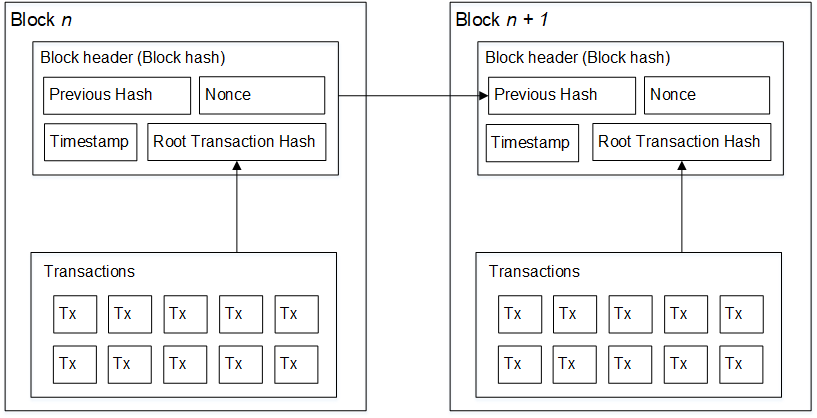
\includegraphics[width=.95\textwidth]{blocks-bitcoin}
    \caption{}
    \label{fig:blocks-bitcoin}
\end{figure}

\subsubsection{Alt-coins}

% Maybe mention slightly